% ----- formatovani dokumentu -----------------------------------------------
\documentclass[12pt,a4paper,titlepage,final]{report}
\usepackage[utf8]{inputenc}
\usepackage[T1, IL2]{fontenc}
\usepackage{graphicx}
\usepackage{epstopdf}
\usepackage[margin=2cm]{caption}
\usepackage[top=3cm, left=2cm, right=2cm, text={17cm, 24cm}, ignorefoot]{geometry}
\usepackage[usenames,dvipsnames]{color}
\usepackage[]{algorithm2e}
\usepackage{amsmath}

% ------ commands -----------------------


% ---------------------------------------

\usepackage{url}
\usepackage{setspace}
\singlespacing
\usepackage[square, numbers]{natbib} 
\pagestyle{plain}
\pagenumbering{arabic}
\setcounter{page}{1}

\setlength{\parindent}{1cm}	
\usepackage{natbib}
\renewcommand{\thesection}{\arabic{section}}
\renewcommand{\thesubsection}{\arabic{section}.\arabic{subsection}}



% ----- vyberte jazyk -------------------------------------------------------
\usepackage[english,czech]{babel}
%\usepackage[english]{babel}

% ----- dopiste titulky -----------------------------------------------------
\newcommand\Course{Geografické informační systémy}
\newcommand\WorkTitle{Rastrové a vektorové analýzy}
\newcommand\AuthorA{Pavel Macenauer}
\newcommand\AuthorAEmail{xmacen02@stud.fit.vutbr.cz}
\newcommand\Faculty{Fakulta Informačních Technologií}
\newcommand\School{Vysoké Učení Technické v~Brně}

\usepackage[
pdftitle={\WorkTitle},
pdfauthor={\AuthorA},
bookmarks=true,
colorlinks=true,
breaklinks=true,
urlcolor=blue,
citecolor=blue,
linkcolor=blue,
unicode=true,
]
{hyperref}



% ----- titulni strana ------------------------------------------------------

\begin{document}
	\begin{titlepage}
	\begin{center}
		\includegraphics[height=5cm]{images/logo.eps}
	\end{center}
	\vfill
	\begin{center}
		\begin{Large}
			\Course\\
		\end{Large}
		\bigskip
		\begin{Huge}
			\WorkTitle\\
		\end{Huge}
	\end{center}
	\vfill
	\begin{center}
		\begin{large}
			\today
		\end{large}
	\end{center}
	\vfill
	\begin{flushleft}
		\begin{large}
			\begin{tabular}{lll}
				Autor: & \AuthorA, & \url{\AuthorAEmail} \\
		
				& & \\
				& \Faculty \\
				& \School \\
			\end{tabular}
		\end{large}
	\end{flushleft}
\end{titlepage}		

\tableofcontents

% ----- obsah -------------------------------------------------------------
\newpage

\section{Cíl práce}

Cílem této práce je vybrat si, nastudovat a naimplementovat několik netriviální rastrových nebo vektorových analytických metod. Vybrány byly metody slope, drain a shaded relief, tedy metody pro svah, odtok vody a reliéf krajiny.

\section{Implementace}

Nástroj pro rastrové analýzy je naimplementován v jazyce \verb|C++| se závislostí na knihovnu \verb|GDAL|\footnote{Geospatial Data Abstraction Library, \url{http://www.gdal.org/}}, open-sourcové knihovně pro čtení a zápis rastrových GIS formátů.

\section{Rastrové metody}

\subsection{Slope}\label{subsec:slope}

Strmost svahu se pro každou buňku počítá na 3x3 uzemí v okolí dané buňky, kde pokud je některá buňka tohoto území nedefinovaná (typicky na okrajích), je výsledná hodnota určena jako 0.

Vzorec pro výpočet svahu kombinuje změnu nadmořské výšky v horizontálním (východ-západ) a vertikálním směru (jih-sever) a to následovně:

\begin{eqnarray}
	slope_{rad} &=& arctg(\sqrt{(\frac{dz}{dx})^2 + (\frac{dz}{dy})^2})
\end{eqnarray}

V praxi je vzorec implementován jako rozdíl hodnot vrchních a spodních 3 bodů, kde prostřední je započítán 2x, resp. pravých a levých. Pseudokód je popsán v (\ref{fig:pseudo}).

\begin{figure}[ht]
\begin{center}
\begin{verbatim}
	[dz/dx] = ((c + 2f + i) - (a + 2d + g) / (8 * x_resolution)
	[dz/dy] = ((a + 2b + c) - (g + 2h + i) / (8 * y_resolution)
	slope = arctg(sqrt([dz/dx] * [dz/dx] + [dy/dx] * [dy/dx]))
\end{verbatim}
\caption{Pseudokód výpočtu svahu.}
\label{fig:pseudo}
\end{center}
\end{figure}

Hodnoty jsou popsány v (\ref{fig:area}) a \verb|x_resolution|, resp. \verb|y_resolution| značí velikosti/rozlišní buněk v horizontálním, resp. vertikálním směru.

\begin{figure}[ht]
\begin{center}
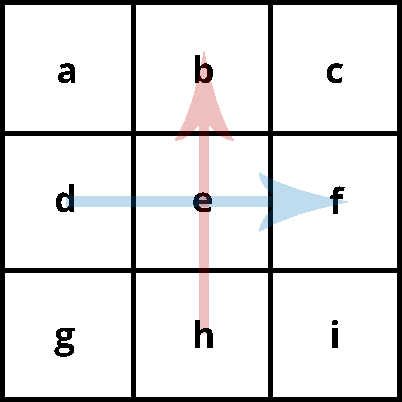
\includegraphics[width=0.20\textwidth]{images/slope.pdf}
\caption{3x3 území pro výpočet strmosti svahu}
\label{fig:area}
\end{center}
\end{figure}

\pagebreak

\subsection{Shaded relief}

Reliéf krajiny se opět vypočte na základě výškové mapy, polohy slunce nad horizontem (0-90 stupňů) a azimutu slunce na východ od severu (0-360 stupňů, ve směru hodinových ručiček). Ve (\ref{eq:relief}) se jedná o \verb|altitude| a \verb|azimuth|.

Nejprve je třeba vypočítat svah a aspekt ve stupních (výpočet svahu je v \ref{subsec:slope}):

\begin{eqnarray*}
slope_{deg} &=& 90 - slope_{rad} \cdot \frac{180}{\pi} \\
aspect &=& arctg(\frac{\frac{dz}{dy}}{\frac{dz}{dx}})
\end{eqnarray*}

Výpočet reliéfu je pak následující:

\begin{eqnarray*}\label{eq:relief}
shaded relief &=& sin(altitude \cdot \frac{\pi}{180}) \cdot sin(slope_{deg} \cdot \frac{\pi}{180}) \\ & & + cos(altitude \cdot \frac{\pi}{180}) \cdot cos(slope_{deg} \cdot \frac{\pi}{180}) \\ & & cos((azimuth - 90) \cdot \frac{\pi}{180} - aspect)
\end{eqnarray*}

\clearpage

\subsection{Drain}

Odtok je rastrová analýza na výškové mapě, která značí kudy by z daného místa odtékala voda, což je nejen užitečné samo o sobě, ale je i základem pro spousty dalších analýz jako zjišťování záplavových oblastí.

Samotný výpočet probíhá tak, že se vždy hledá lokální minimum v okolí daného bodu a to do té doby, dokud existuje, pak se algoritmus zastáví. Jedná se tedy svým způsobem o prohledávání do hloubky.

\begin{figure}[ht]
\begin{center}
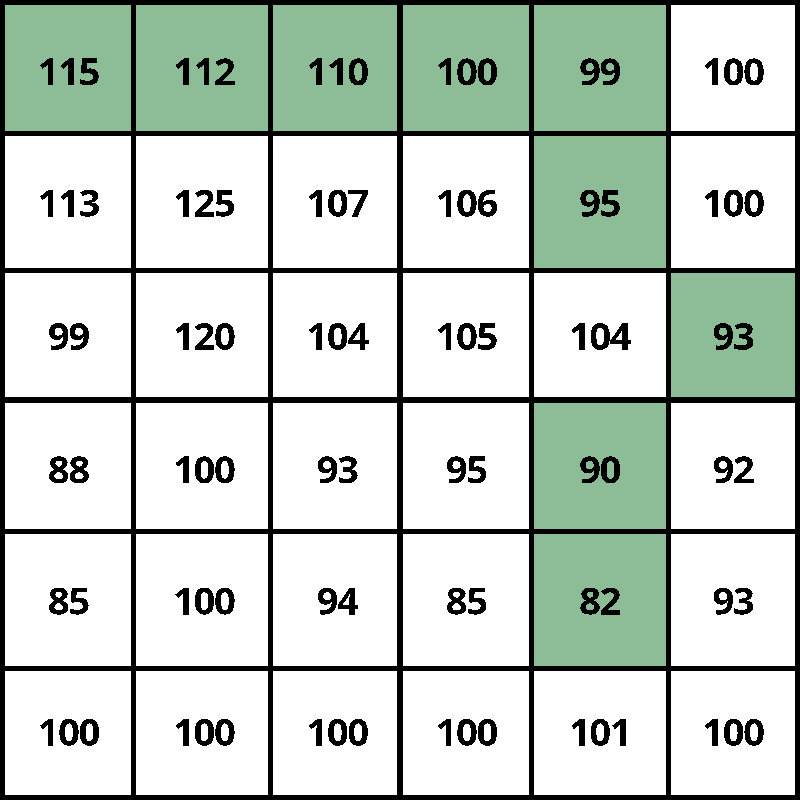
\includegraphics[width=0.4\textwidth]{images/drain.pdf}
\caption{Průběh výpočtu odtoku}
\label{fig:drain}
\end{center}
\end{figure}

Výpočet je ukázán na (\ref{fig:drain}), kdy se vždy najde minimum na okolí 3x3 kolem dané buňky, kde daná hodnota je menší, než hodnota kolem které hledáme. Následně se pokračuje s nalezenou buňkou jako středem a to do té doby, dokud v okolí existuje nějaká menší hodnota. Pokud již neexistuje algoritmus skončí, protože už není kam by voda stékala.

\clearpage

\section{Výsledky}

\begin{itemize}
	\item Repository: \url{https://github.com/mmaci/vutbr-fit-gis-raster-analysis-tool}
	\item Programová dokumentace: \url{http://gis.maciste.cz}
	\item Testovací balíček obsahující potřebné dll, win32 binary a testovací DEM: \url{http://gis.maciste.cz/gistool.zip}
\end{itemize}

\subsection{Možnosti programu}
\begin{verbatim}
-i --input [filename] Input file (supports GeoTiff). (required)
-o --output [filename] Output file. (required)
-m --method [slope/shaded_relief/drain] (required)
-c --coords [filename] Name of input filename with coords for drain method.
-x [number] X-coord for drain method.
-y [number] Y-coord for drain method
\end{verbatim}

\begin{figure}[ht]
\begin{center}
\includegraphics[width=0.9\textwidth]{images/slope_cr.jpg}
\caption{Slope nad celou DEM ČR}
\label{fig:slope-cr}
\end{center}
\end{figure}

\begin{figure}[ht]
\begin{center}
\includegraphics[width=0.5\textwidth]{images/slope_detail.jpg}
\caption{Detail metody slope}
\label{fig:slope-det}
\end{center}
\end{figure}

\begin{figure}[ht]
\begin{center}
\includegraphics[width=0.9\textwidth]{images/sr_cr.jpg}
\caption{Shaded relief nad celou DEM ČR}
\label{fig:slope-cr}
\end{center}
\end{figure}

\begin{figure}[ht]
\begin{center}
\includegraphics[width=0.5\textwidth]{images/sr_detail.jpg}
\caption{Detail metody shaded relief}
\label{fig:slope-det}
\end{center}
\end{figure}

\begin{figure}[ht]
\begin{center}
\includegraphics[width=0.5\textwidth]{images/drain_detail.jpg}
\caption{Detail metody drain, jako vstup je seznam bodů, výstupem jsou jednotlivé odtoky}
\label{fig:slope-cr}
\end{center}
\end{figure}


\bibliographystyle{plain}

\nocite{grass}
\nocite{arcgis}
\nocite{grass-src}
\nocite{freegis}
\nocite{gis-modelling}

\hypertarget{bib}{}
\bibliography{reference}
\addcontentsline{toc}{section}{Literatura}

\end{document}

